\bta{裂变聚变}


\begin{enumerate}
	%\renewcommand{\labelenumi}{\arabic{enumi}.}
	% A(\Alph) a(\alph) I(\Roman) i(\roman) 1(\arabic)
	%设定全局标号series=example	%引用全局变量resume=example
	%[topsep=-0.3em,parsep=-0.3em,itemsep=-0.3em,partopsep=-0.3em]
	%可使用leftmargin调整列表环境左边的空白长度 [leftmargin=0em]
	\item
\exwhere{$ 2019 $ 年物理江苏卷}
$ 100 $ 年前,卢瑟福用$ \alpha $粒子轰击氮核打出了质子.后来,人们用$ \alpha $粒子轰击  \ce{^{60}_{28}Ni} 
核也打出了质子: ${ }_{2}^{4} \mathrm{He}+{ }_{28}^{60} \mathrm{Ni} \rightarrow{ }_{29}^{62} \mathrm{Cu}+{ }_{1}^{1} \mathrm{H}+\mathrm{X}$;该反应中的 $ X $ 是 \underlinegap (选填“电子”“正电子”或“中子”)。此后,对原子核反应的持续研究为核能利用提供了可能.目前人类获得核能的主要方式是
 \underlinegap 
(选填“核衰变”“核裂变”或“核聚变”)。

 \tk{中子 \quad 核裂变} 




\item
\exwhere{$ 2014 $ 年物理上海卷}
链式反应中,重核裂变时放出的可以使裂变不断进行下去的粒子是 \xzanswer{B} 

\fourchoices
{质子}
{中子}
{$ \beta $粒子}
{$ \alpha $粒子}




\item 
\exwhere{$ 2013 $ 年重庆卷}
铀是常用的一种核燃料,若它的原子核发生了如下的裂变反应:${ }_{92}^{235} \mathrm{U}+{ }_{0}^{1} \mathrm{n} \rightarrow a+b+2{ }_{0}^{1} \mathrm{n}$。则 $ a+b $ 可能是 \xzanswer{D} 

\fourchoices
{${ }_{54}^{140} \mathrm{Xe}+{ }_{36}^{93} \mathrm{Kr}$}
{${ }_{56}^{141} \mathrm{Ba}+{ }_{36}^{92} \mathrm{Kr}$}
{${ }_{56}^{141} \mathrm{Ba}+{ }_{38}^{93} \mathrm{Sr}$}
{${ }_{54}^{140} \mathrm{Xe}+{ }_{38}^{94} \mathrm{Sr}$}



\item 
\exwhere{$ 2013 $ 年广东卷}
铀核裂变是核电站核能的重要来源,其一种裂变反应是
${ }_{92}^{235} \mathrm{U}+{ }_{0}^{1} \mathrm{n} \rightarrow{ }_{56}^{144} \mathrm{Ba}+{ }_{36}^{89} \mathrm{Kr}+3{ }_{0}^{1} \mathrm{n}$
下列说法正确的有 \xzanswer{AC} 

\fourchoices
{上述裂变反应中伴随着中子放出}
{铀块体积对链式反应的发生无影响}
{铀核的链式反应可人工控制}
{铀核的半衰期会受到环境温度的影响}



\item 
\exwhere{$ 2015 $ 年上海卷}
铀核可以发生衰变和裂变,铀核的 \xzanswer{C} 


\fourchoices
{衰变和裂变都能自发发生}
{衰变和裂变都不能自发发生}
{衰变能自发发生而裂变不能自发发生}
{衰变不能自发发生而裂变能自发发生}

\item 
\exwhere{$ 2017 $ 年天津卷}
我国自主研发制造的国际热核聚变核心部件在国际上率先通过权威机构认证,
这是我国对国际热核聚变项目的重大贡献。下列核反应方程中属于聚变反应的是 \xzanswer{A} 
% TODO: \usepackage{graphicx} required
\begin{figure}[h!]
	\centering
	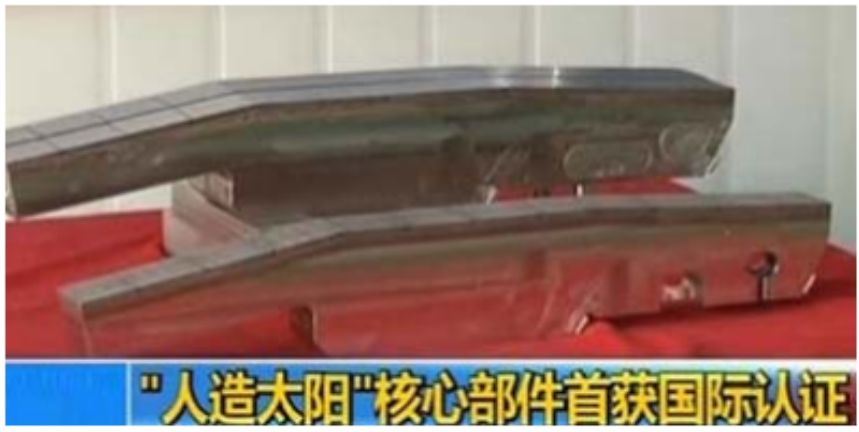
\includegraphics[width=0.27\linewidth]{picture/screenshot071}
\end{figure}


\fourchoices
{${ }_{1}^{2} \mathrm{H}+{ }_{1}^{3} \mathrm{H} \rightarrow{ }_{2}^{4} \mathrm{He}+{ }_{0}^{1} \mathrm{n}$}
{${ }_{7}^{14} \mathrm{~N}+{ }_{2}^{4} \mathrm{He} \rightarrow{ }_{8}^{17} \mathrm{O}+{ }_{1}^{1} \mathrm{H}$}
{${ }_{2}^{4} \mathrm{He}+{ }_{13}^{27} \mathrm{Al} \rightarrow{ }_{15}^{30} \mathrm{P}+{ }_{0}^{1} \mathrm{n}$}
{${ }_{92}^{235} \mathrm{U}+{ }_{0}^{1} \mathrm{n} \rightarrow{ }_{56}^{144} \mathrm{Ba}+{ }_{36}^{89} \mathrm{Kr}+3{ }_{0}^{1} \mathrm{n}$}


	
	
	
\end{enumerate}

